\documentclass[11pt,a4paper]{article}

\usepackage[T1]{fontenc}
\usepackage{lmodern}
\usepackage[margin=2.5cm]{geometry}
\usepackage{amsmath,amssymb}
\usepackage{booktabs}
\usepackage{graphicx}
\usepackage{caption}
\usepackage{microtype}
\usepackage[numbers,sort&compress]{natbib}
\usepackage[hidelinks]{hyperref}
\usepackage{xcolor}

\graphicspath{{../figures/}{figures/}}
\captionsetup{font=small,labelfont=bf}
% Generated by scripts/11_paper_assets.py -- do not edit by hand.
\newcommand{\acqBestDv}{1.12}
\newcommand{\acqBestRho}{3.2}
\newcommand{\cheapDist}{69}
\newcommand{\cheapDv}{1.11}
\newcommand{\cheapRho}{1.8}
\newcommand{\coastAcqDays}{61}
\newcommand{\coastHoldDaysMax}{314}
\newcommand{\coastHoldDaysMean}{250}
\newcommand{\coastHoldDaysMin}{222}
\newcommand{\cubAcqDv}{$1.46 \pm 0.18$}
\newcommand{\cubAcqRatioMax}{1.4}
\newcommand{\cubAcqRatioMin}{1.1}
\newcommand{\cubBestMax}{250k}
\newcommand{\cubBestMin}{200k}
\newcommand{\cubHoldDist}{$0.57 \pm 0.17$}
\newcommand{\cubHoldDv}{$0.110 \pm 0.007$}
\newcommand{\cubHoldRatio}{$1.87 \pm 0.77$}
\newcommand{\cubRatioMax}{2.7}
\newcommand{\cubRatioMin}{1.3}
\newcommand{\cubicActionForHold}{0.12}
\newcommand{\dqnAcqDv}{2.17}
\newcommand{\dqnHoldDist}{1.4}
\newcommand{\dqnHoldDv}{0.72}
\newcommand{\dqnOneBig}{0}
\newcommand{\dqnOneCoast}{0}
\newcommand{\dqnOneMid}{14}
\newcommand{\dqnOneSmall}{351}
\newcommand{\dqnRatioMax}{12}
\newcommand{\dqnRatioMin}{2}
\newcommand{\dqnSteps}{1M}
\newcommand{\dqnTwoBig}{0}
\newcommand{\dqnTwoCoast}{214}
\newcommand{\dqnTwoMid}{97}
\newcommand{\dqnTwoSmall}{54}
\newcommand{\efoldDays}{23.0}
\newcommand{\holdDistMax}{2.5}
\newcommand{\holdDistMin}{0.4}
\newcommand{\holdDvMax}{0.95}
\newcommand{\holdDvMin}{0.03}
\newcommand{\lOneDistKm}{1{,}491{,}539}
\newcommand{\lambdaU}{2.533}
\newcommand{\linAcqDv}{$1.72 \pm 0.12$}
\newcommand{\linBestMax}{2.95M}
\newcommand{\linBestMin}{1.2M}
\newcommand{\linCubAcqMax}{1.3}
\newcommand{\linCubAcqMin}{1.1}
\newcommand{\linCubHoldMax}{4.1}
\newcommand{\linCubHoldMin}{3.1}
\newcommand{\linHoldDist}{$0.45 \pm 0.04$}
\newcommand{\linHoldDv}{$0.393 \pm 0.039$}
\newcommand{\linHoldRatio}{$4.43 \pm 1.51$}
\newcommand{\linearActionForHold}{2\times10^{-3}}
\newcommand{\lqrAcqDist}{76}
\newcommand{\lqrAcqDv}{1.12}
\newcommand{\lqrHoldDist}{0.52}
\newcommand{\lqrHoldDv}{0.062}
\newcommand{\lqrPeakFive}{4.9\times10^{-6}}
\newcommand{\muSE}{3.0034\times10^{-6}}
\newcommand{\noiseLost}{0}
\newcommand{\noiseOverHiMax}{5.6}
\newcommand{\noiseOverHiMin}{4.0}
\newcommand{\noiseOverNomMax}{1.9}
\newcommand{\noiseOverNomMin}{1.7}
\newcommand{\ppoEnvs}{8}
\newcommand{\ppoSteps}{3M}
\newcommand{\ppoThreeDv}{13}
\newcommand{\ppoThreeLateMax}{215}
\newcommand{\ppoThreeLateMin}{56}
\newcommand{\pullFive}{1.3\times10^{-6}}
\newcommand{\pullThree}{7.6\times10^{-7}}
\newcommand{\rhoCount}{19}
\newcommand{\rhoDecades}{9}
\newcommand{\satLostThree}{10}
\newcommand{\sweepRhoCount}{57}
\newcommand{\thrDays}{365}
\newcommand{\thrLinBig}{185}
\newcommand{\thrLinMedian}{1.0\times10^{-8}}
\newcommand{\thrLqrBig}{0}
\newcommand{\thrLqrMedian}{1.79\times10^{-9}}
\newcommand{\thrPpoBig}{27}
\newcommand{\thrPpoMedian}{1.73\times10^{-9}}
\newcommand{\tuDays}{58.13}
\newcommand{\wFuel}{10}
\newcommand{\wPos}{0.3}


\newcommand{\dv}{\Delta v}
\newcommand{\todo}[1]{\textcolor{red}{[TODO: #1]}}

\title{Is Reinforcement Learning Cheaper than LQR?\\[0.3em]
\large Fuel-Efficient Station-Keeping at the Unstable Sun--Earth $L_1$ Point}
\author{Emir Eymen Sarg\i n\\
\small TEV \.{I}nan\c{c} Lisesi, Kocaeli, T\"urkiye}
\date{Draft, \today}

\begin{document}
\maketitle

\begin{abstract}
A spacecraft at the Sun--Earth $L_1$ point drifts away exponentially, with an
$e$-folding time of \efoldDays~days, unless it fires its thrusters regularly.
We ask whether a deep reinforcement learning (RL) agent can hold it there with
less fuel than a linear--quadratic regulator (LQR). All controllers fly the same
nonlinear planar circular restricted three-body model with navigation errors,
thrust errors and unmodelled forces, and are scored on 20 held-out random
seeds. A DQN agent with 25 discrete actions keeps the spacecraft in every test
episode but needs \dqnRatioMin--\dqnRatioMax$\times$ the fuel of LQR. With a
continuous action and a cubic thrust map, PPO reaches the right thrust scale and
spends \cubHoldDv~m/s per year while holding (LQR: \lqrHoldDv~m/s). Comparing
against LQR tuned to the \emph{same} tracking accuracy, PPO needs
\cubRatioMin--\cubRatioMax$\times$ LQR's fuel across three training seeds and
never reaches the LQR fuel--accuracy curve. Most of the DQN--LQR gap therefore
came from the action representation, not from learning, but LQR remains
Pareto-optimal. Two single-run findings did not survive retraining with new
seeds, including an apparent advantage of PPO under a thrust limit; we report
them as a cautionary example. Code and data are open source.
\end{abstract}

% ===========================================================================
\section{Introduction}

The collinear Lagrange points $L_1$ and $L_2$ of the Sun--Earth system are
attractive places for observatories: SOHO watches the Sun from $L_1$, and JWST
observes from near $L_2$. Both points are equilibria of the circular restricted
three-body problem (CR3BP), but unstable ones \cite{szebehely1967,koon2011}. A
spacecraft left exactly at $L_1$ with a 150~m error drifts away by a factor $e$
every \efoldDays~days and is more than a million kilometres away within a year
(Fig.~\ref{fig:escape}). Missions therefore perform \emph{station-keeping}: small,
regular thruster firings that cancel the unstable motion
\cite{farquhar1970,howell1993}.

Classical station-keeping uses linear control around the reference. Recently,
deep reinforcement learning has been applied to guidance and station-keeping in
multi-body dynamics \cite{lafarge2021,lafarge2022,molnar2020,suda2023}, often
with promising results. Our question is narrower and deliberately simple:
\begin{quote}
\emph{On the most basic station-keeping problem, holding the $L_1$ point
itself, can a learned controller beat LQR on fuel at the same tracking
accuracy?}
\end{quote}
We expected LQR to be hard to beat, because the motion stays in a region where
the linearised dynamics are very accurate and LQR is the optimal controller for
linear dynamics and quadratic cost. The value of the experiment is in measuring
\emph{how close} RL gets, and \emph{why} it falls short.

Our contributions are:
\begin{enumerate}
\item A from-scratch CR3BP simulator with a shared station-keeping environment,
      so that LQR and RL see identical physics, errors and fuel accounting, and
      a fixed test protocol on seeds never used in training or model selection.
\item A fair comparison: each learned controller is compared with LQR tuned to
      the same tracking accuracy, interpolated on a 57-point LQR sweep.
\item Evidence that the action representation, not the learning algorithm, is
      the main reason DQN needs much more fuel: a continuous PPO agent with a
      cubic thrust map reduces the gap from \dqnRatioMin--\dqnRatioMax$\times$
      to \cubRatioMin--\cubRatioMax$\times$.
\item A seed study showing which conclusions hold across training seeds and
      which do not \cite{henderson2018,agarwal2021}.
\end{enumerate}

% ===========================================================================
\section{Model}

\subsection{Circular restricted three-body problem}

We use the standard nondimensional units: the Sun--Earth distance is 1, the
total mass is 1 and the Earth's orbital period is $2\pi$, so one time unit is
\tuDays~days. The mass ratio is $\mu = m_E/(m_S + m_E) = \muSE$. In the frame
rotating with the Earth, with the Sun at $(-\mu, 0)$ and the Earth at
$(1-\mu, 0)$, the planar equations of motion with a control acceleration
$\mathbf{u} = (u_x, u_y)$ are
\begin{equation}
\ddot{x} - 2\dot{y} = \frac{\partial \Omega}{\partial x} + u_x, \qquad
\ddot{y} + 2\dot{x} = \frac{\partial \Omega}{\partial y} + u_y, \qquad
\Omega = \frac{x^2 + y^2}{2} + \frac{1-\mu}{r_1} + \frac{\mu}{r_2},
\label{eq:cr3bp}
\end{equation}
where $r_1$ and $r_2$ are the distances to the Sun and the Earth. With
$\mathbf{u} = 0$ the Jacobi constant $C = 2\Omega - \dot{x}^2 - \dot{y}^2$ is
conserved, which we use to validate the integrators. Over ten years, the
adaptive DOP853 integrator \cite{hairer1993} keeps the relative error in $C$
below $10^{-13}$, and the fixed-step RK4 integrator used inside the simulator
converges with a measured order of 3.92 (theory: 4).

\subsection{Lagrange points and linear stability}

The collinear points are the roots of $\partial\Omega/\partial x = 0$ on the
$x$ axis. Linearising Eq.~\eqref{eq:cr3bp} about a point gives
$\dot{\mathbf{x}} = A\mathbf{x}$ with $\mathbf{x} = (\delta x, \delta y,
\delta\dot{x}, \delta\dot{y})$. At $L_1$ the eigenvalues of $A$ are a saddle
pair $\pm\lambda$ and a centre pair $\pm i\omega$, with $\lambda = \lambdaU$
(Table~\ref{tab:lagrange}). The saddle makes $L_1$ unstable: a small error
grows like $e^{\lambda t}$. Without control, a spacecraft that starts 1000~km
from $L_1$ is more than $10^4$~km away after \coastAcqDays~days, and even one
that starts exactly at $L_1$ is pushed out by the unmodelled forces of
Section~\ref{sec:errors} within \coastHoldDaysMin--\coastHoldDaysMax~days.

\begin{table}[t]
\centering
\caption{Sun--Earth Lagrange points computed by the simulator.
$\lambda$ is the largest real part of the eigenvalues of $A$, in nondimensional
units; the $e$-folding time is $1/\lambda$ in days.}
\label{tab:lagrange}
\begin{tabular}{llll}
\toprule
Point & Distance from Earth & Unstable eigenvalue $\lambda$ & $e$-folding time \\
\midrule
L1 & 1{,}491{,}539~km & 2.533 & 23.0 days \\
L2 & 1{,}501{,}519~km & 2.484 & 23.4 days \\
L3 & 299{,}195{,}479~km & 0.0028 & 57 years \\
L4, L5 & 1 AU (60\textdegree{} ahead/behind) & 0 & stable (Routh: $\mu < 0.0385$) \\
\bottomrule
\end{tabular}

\end{table}

\begin{figure}[t]
\centering
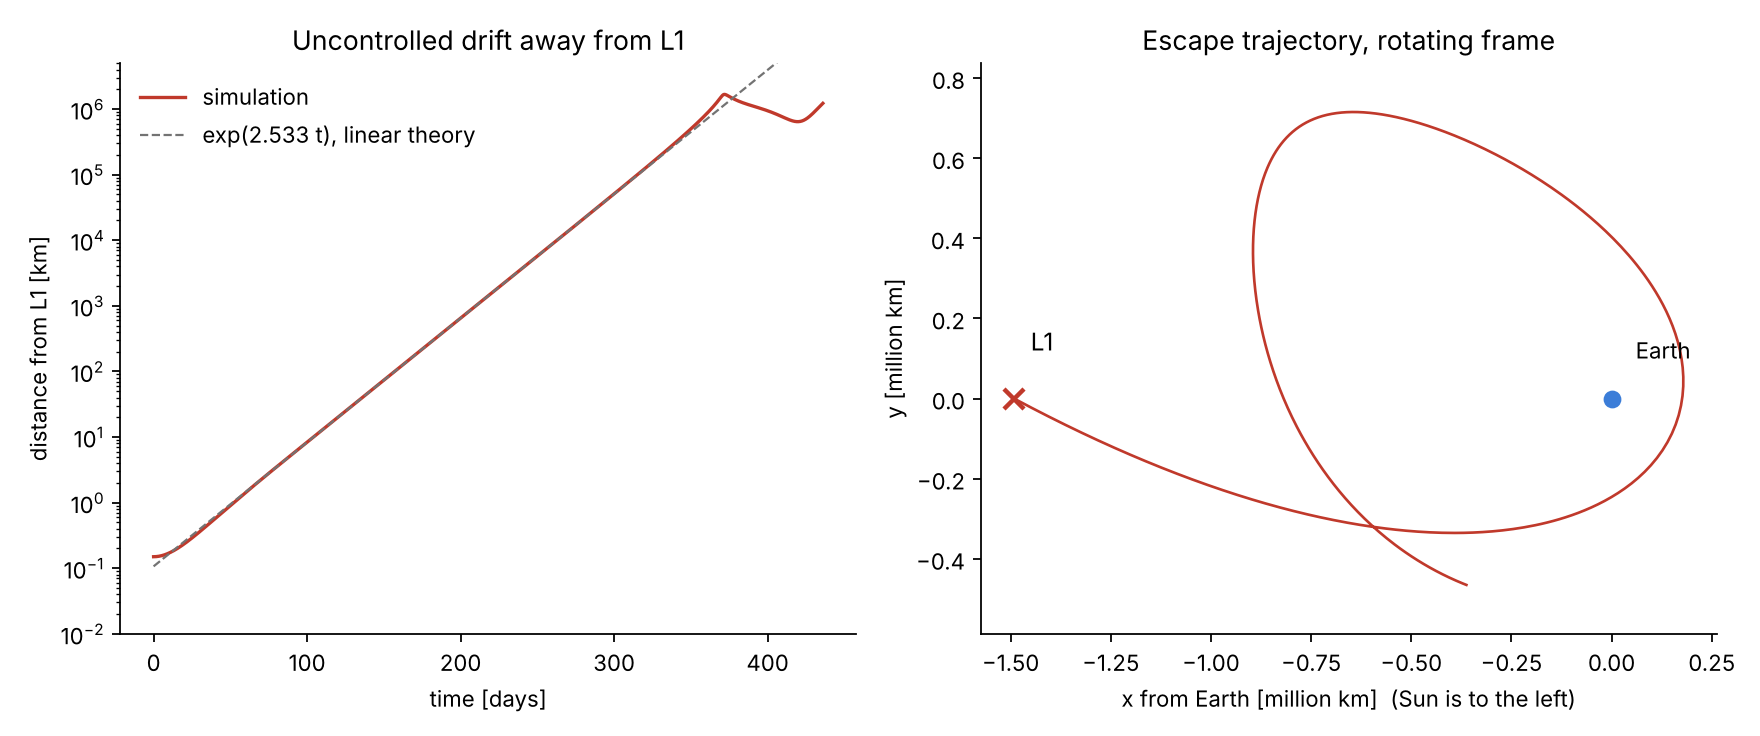
\includegraphics[width=\linewidth]{l1_escape}
\caption{Uncontrolled drift from $L_1$, starting 150~m away at rest. Left: the
distance grows at the rate predicted by the unstable eigenvalue. Right: the
escape trajectory in the rotating frame.}
\label{fig:escape}
\end{figure}

% ===========================================================================
\section{The station-keeping problem}
\label{sec:problem}

\paragraph{Simulator.}
The spacecraft follows the full nonlinear dynamics \eqref{eq:cr3bp}. Once per
day a controller reads a noisy estimate of its position and velocity relative
to $L_1$ and commands a thrust acceleration, which is held constant for the
day (zero-order hold). Fuel is measured as the total velocity change actually
delivered, $\dv = \sum_k \lVert \mathbf{u}_k \rVert \, \Delta t$. An episode
lasts one year; the spacecraft is \emph{lost} if it is ever more than
10\,000~km from $L_1$.

\paragraph{Error model.}
\label{sec:errors}
Every controller faces the same errors (1$\sigma$, independent per axis and per
day, drawn from the same random seed for every controller): navigation errors of
1~km in position and 1~mm/s in velocity; a thrust magnitude error of 2\,\% and
a pointing error of 1\textdegree; and an unmodelled acceleration of
$10^{-9}$~m/s$^2$, which stands in for changes in solar radiation pressure and
the pull of the Moon and planets. These values are illustrative assumptions for
a deep-space mission, not those of a specific spacecraft.

\paragraph{Scenarios and metrics.}
\emph{Holding}: the spacecraft starts at $L_1$ at rest.
\emph{Recovery}: it starts 1000~km away on the Sun--Earth line. For each
episode we record $\dv$ over the year, the mean and RMS distance from $L_1$,
and whether the spacecraft was kept for the full year.

\paragraph{Test protocol.}
During training and model selection, agents are only ever evaluated on seeds
0--4. All results in this paper use seeds 100--119, which are never touched
until the final evaluation. Because the seed fixes every random draw, all
controllers meet exactly the same navigation errors, thrust errors and
disturbances, draw for draw.

\paragraph{Simplifications.}
Real $L_1$ missions fly halo or Lissajous orbits around the point rather than
holding the point itself, the motion is three-dimensional, and manoeuvres are
usually impulsive and weeks apart. We keep the problem planar, hold the point,
and use a small daily thrust so that the comparison between controllers is
clean; Section~\ref{sec:limits} discusses what this means for the conclusions.

% ===========================================================================
\section{Controllers}

\subsection{LQR baseline}

Because the thrust is constant over each day, the linear model can be
discretised exactly with a zero-order hold, $\mathbf{x}_{k+1} = A_d \mathbf{x}_k
+ B_d \mathbf{u}_k$, where $A_d$ and $B_d$ come from one matrix exponential.
The LQR gain $K$ minimises $\sum_k \mathbf{x}_k^\top Q \mathbf{x}_k +
\mathbf{u}_k^\top R \mathbf{u}_k$ and follows from the discrete algebraic
Riccati equation \cite{bryson1975}. We set the weights with Bryson's rule,
\begin{equation}
Q = \operatorname{diag}\!\left(\tfrac{1}{r_\text{ref}^2}, \tfrac{1}{r_\text{ref}^2},
\tfrac{1}{v_\text{ref}^2}, \tfrac{1}{v_\text{ref}^2}\right), \qquad
R = \frac{\rho}{u_\text{ref}^2} I_2,
\end{equation}
with $r_\text{ref} = 1000$~km, $v_\text{ref} = 1$~m/s and $u_\text{ref} =
10^{-6}$~m/s$^2$, and vary the single fuel weight $\rho$: a larger $\rho$ means
less thrust and looser tracking. The controller is $\mathbf{u}_k = -K
\hat{\mathbf{x}}_k$, applied directly to the noisy estimate $\hat{\mathbf{x}}_k$
without a filter. As a reference we use $\rho = 3$, the cheapest recovery in an
initial sweep.

\subsection{Reinforcement learning environment}

The RL agents fly the same simulator through a Gymnasium interface. The
observation has 8 values computed from the noisy estimate: position in units of
1000~km, velocity in m/s, and the symmetric logarithm
$\operatorname{sign}(z)\log_{10}(1 + |z|)$ of the position in km and the
velocity in mm/s, so that both 0.1~km and 1000~km are visible to the network.
The reward per day is
\begin{equation}
r_k = 1 - w_\text{pos}\log_{10}\!\left(1 + \frac{d_k}{1~\text{km}}\right)
- w_\text{fuel}\,\frac{\dv_k}{1~\text{m/s}} - 100\cdot\mathbb{1}[\text{lost}],
\end{equation}
with $d_k$ the distance from $L_1$, $w_\text{pos} = \wPos$ and $w_\text{fuel} =
\wFuel$. Training episodes start at a random offset of up to 1000~km with a
small random velocity, so both holding and recovery are learned.

\paragraph{DQN (discrete thrust).}
DQN \cite{mnih2015} chooses each day one of 25 actions: coast, or thrust in one
of 8 directions at $10^{-8}$, $10^{-7}$ or $10^{-6}$~m/s$^2$. We trained two
runs of \dqnSteps\ steps; run~2 uses a lower learning rate, slower target
updates and a stronger distance penalty after run~1 became unstable late in
training.

\paragraph{PPO (continuous thrust).}
PPO \cite{schulman2017} outputs a two-dimensional action $\mathbf{a}$ with
$\lVert\mathbf{a}\rVert \leq 1$, which is mapped to thrust by
\begin{equation}
\mathbf{u} = u_\text{max}\,\lVert\mathbf{a}\rVert^{p-1}\,\mathbf{a},
\qquad u_\text{max} = 10^{-6}~\text{m/s}^2,
\label{eq:actionmap}
\end{equation}
the same limit as DQN's largest action. With the plain linear map ($p = 1$),
the holding thrust LQR uses (about $2\times10^{-9}$~m/s$^2$) corresponds to an
action of norm $\linearActionForHold$, a value the Gaussian policy struggles to
output precisely. With the cubic map ($p = 3$) the same thrust needs
$\lVert\mathbf{a}\rVert \approx \cubicActionForHold$, while the full thrust is
still available. We train both maps to isolate this choice.

\paragraph{Training and model selection.}
Both algorithms use the Stable-Baselines3 implementations \cite{raffin2021}
with the hyperparameters in Table~\ref{tab:hyper}. Every 25\,000 (DQN) or
50\,000 (PPO) steps, the deterministic policy flies holding and recovery on
seeds 0--4 and is scored by
$\frac{1}{2}\sum_\text{scen} \bigl(100\,\tfrac{\text{days kept}}{365} -
10\,\dv - \log_{10}(1 + \bar{d})\bigr)$; the best checkpoint of each run is
kept. Each PPO configuration was trained with three training seeds (0, 1, 2)
and otherwise identical settings, \ppoSteps\ steps each with \ppoEnvs\ parallel
environments (about 11~minutes on one CPU core per run).

\begin{table}[t]
\centering
\caption{Training hyperparameters (Stable-Baselines3).}
\label{tab:hyper}
\small
\begin{tabular}{ll@{\hskip 2.5em}ll}
\toprule
\multicolumn{2}{c}{DQN (run 2)} & \multicolumn{2}{c}{PPO} \\
\midrule
Steps & $10^6$ & Steps & $3\times10^6$ (8 envs) \\
Learning rate & $10^{-4}$ & Learning rate & $3\times10^{-4}$ \\
Replay buffer & $2\times10^5$ & Rollout per env & 512 \\
Batch size & 256 & Batch size / epochs & 256 / 10 \\
Target update & every $10^4$ steps & GAE $\lambda$ / clip & 0.95 / 0.2 \\
Exploration & $\varepsilon$: 1 $\to$ 0.02 over 30\,\% & Initial log std & $-1$ \\
Network & 128--128 & Networks (policy, value) & 128--128 each \\
$\gamma$ & 0.99 & $\gamma$ & 0.99 \\
\bottomrule
\end{tabular}
\end{table}

% ===========================================================================
\section{Results}

\subsection{The LQR fuel--accuracy trade-off}

Sweeping $\rho$ over \rhoDecades\ orders of magnitude (Fig.~\ref{fig:pareto})
shows the trade-off the agents must beat. While holding, LQR spends
\holdDvMin--\holdDvMax~m/s per year for a mean distance of
\holdDistMax--\holdDistMin~km. Below about 0.4~km the navigation error sets a
floor and extra fuel buys almost nothing. For recovery the curve is not
monotonic: the cheapest gain ($\rho \approx \acqBestRho$, \acqBestDv~m/s) sits
in the middle, and \emph{lazier} gains cost \emph{more}, because the unstable
mode keeps growing while the controller waits.

\begin{figure}[t]
\centering
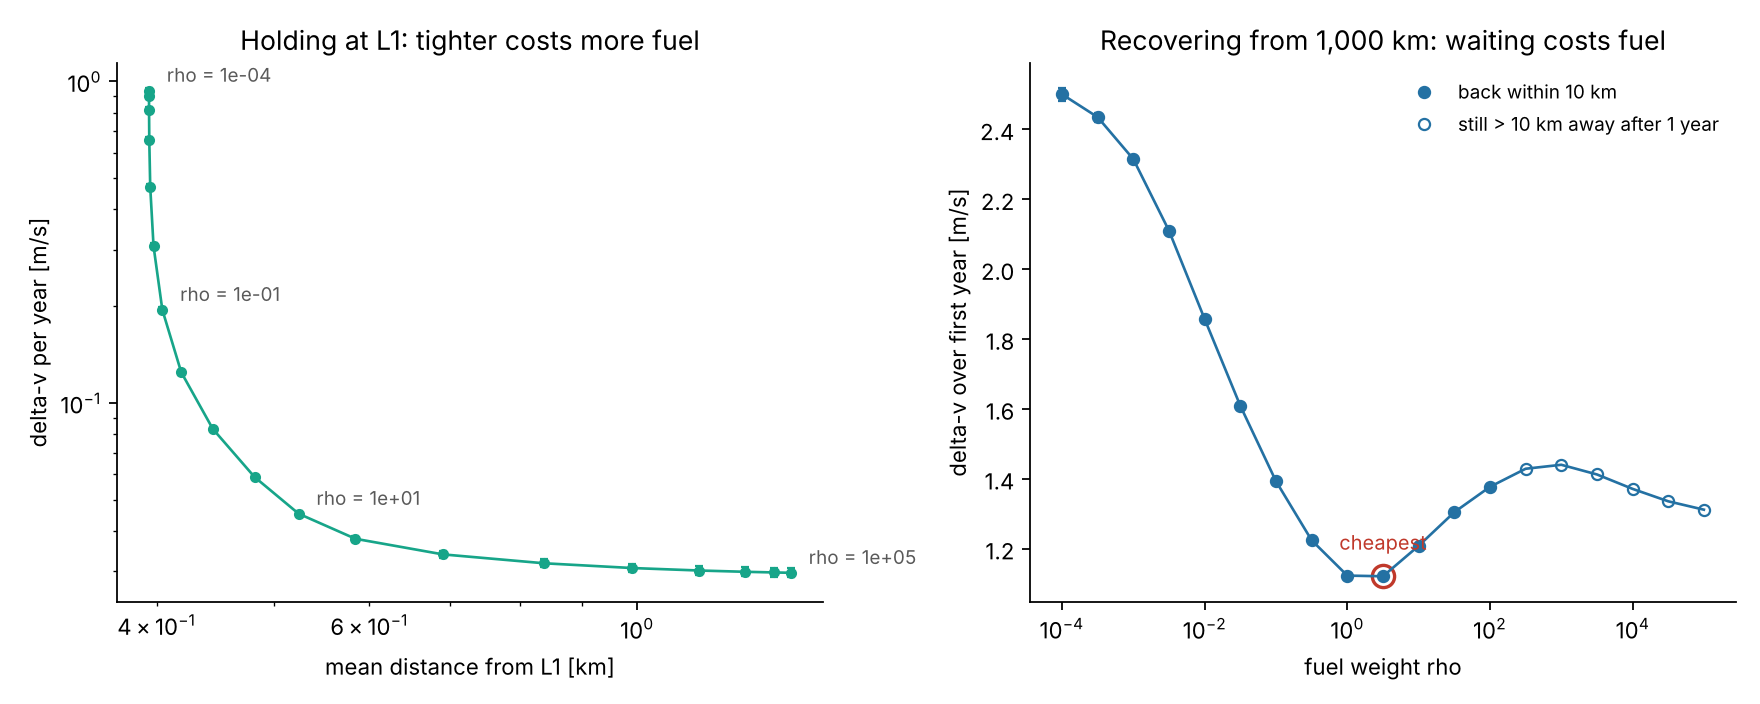
\includegraphics[width=\linewidth]{lqr_pareto}
\caption{LQR fuel versus tracking accuracy as the fuel weight $\rho$ is varied
(5 seeds per point). Left: holding. Right: recovery from 1000~km.}
\label{fig:pareto}
\end{figure}

\subsection{Main comparison}

Table~\ref{tab:main} summarises the test results. Every learned controller
keeps the spacecraft in every test episode, so the question is purely one of
fuel and accuracy. DQN needs \dqnRatioMin--\dqnRatioMax$\times$ the fuel of
LQR. PPO with the cubic map spends \cubHoldDv~m/s while holding, much closer to
LQR's \lqrHoldDv~m/s, and the linear map lies in between.

\begin{table}[t]
\centering
\caption{Test results (seeds 100--119). PPO rows are mean $\pm$ standard
deviation over three training seeds; ``Kept'' is the share of episodes kept for
the full year.}
\label{tab:main}
\small
\setlength{\tabcolsep}{3pt}
\begin{tabular}{lccccc}
\toprule
& \multicolumn{2}{c}{Holding (start at L1)} & \multicolumn{2}{c}{Recovery (start 1000 km)} & \\
\cmidrule(lr){2-3}\cmidrule(lr){4-5}
Controller & $\Delta v$ [m/s] & mean / RMS dist.\ [km] & $\Delta v$ [m/s] & mean dist.\ [km] & Kept \\
\midrule
No control & 0 & lost after 250 d & 0 & lost after 61 d & 0\,\% \\
LQR, $\rho = 3$ & 0.062 & 0.52 / 0.59 & 1.12 & 76 & 100\,\% \\
DQN (run 2, seed 0) & 0.723 & 1.41 / 1.62 & 2.17 & 68 & 100\,\% \\
PPO, linear map ($p=1$) & $0.393 \pm 0.039$ & $0.45 \pm 0.04$ / $0.51 \pm 0.04$ & $1.72 \pm 0.12$ & $72 \pm 14$ & 100\,\% \\
PPO, cubic map ($p=3$) & $0.110 \pm 0.007$ & $0.57 \pm 0.17$ / $0.64 \pm 0.18$ & $1.46 \pm 0.18$ & $84 \pm 30$ & 100\,\% \\
\bottomrule
\end{tabular}

\end{table}

\subsection{Fair comparison at the same accuracy}

The agents do not track at exactly the accuracy of LQR with $\rho = 3$, and
fuel can always be traded for accuracy. We therefore compare each model with
LQR tuned to the same mean distance. LQR is swept over \sweepRhoCount\ values
of $\rho$ between $10^{-3}$ and $10^4$ on the test seeds. Along the sweep,
tighter tracking costs more fuel only up to the $\dv$ minimum; beyond it,
lazier gains cost more again, so only this left branch is a sensible reference.
On it we interpolate (log--log) the LQR fuel at the model's mean distance and
report the ratio. If a model is \emph{less} accurate than the cheapest LQR
($\rho \approx \cheapRho$: \cheapDv~m/s at \cheapDist~km in recovery), that LQR
is both cheaper and more accurate; we call the model \emph{dominated} and give
the ratio to the cheapest LQR as a lower bound.

\begin{table}[t]
\centering
\caption{Fuel of each PPO model divided by the fuel of LQR tuned to the same
mean distance (test seeds). ``Best checkpoint'' is the training step of the
selected model.}
\label{tab:ratio}
\small
\begin{tabular}{llccc}
\toprule
Thrust map & Training seed & Holding & Recovery & Best checkpoint \\
\midrule
cubic & 0 & 1.54 & 1.44 & 250k \\
cubic & 1 & 1.31 & 1.13 & 250k \\
cubic & 2 & 2.74 & dominated ($\geq 1.37$) & 200k \\
\addlinespace
linear & 0 & 4.48 & 1.61 & 2.95M \\
linear & 1 & 5.92 & dominated ($\geq 1.48$) & 1.20M \\
linear & 2 & 2.90 & dominated ($\geq 1.50$) & 2.90M \\
\addlinespace
cubic & mean $\pm$ std & $1.87 \pm 0.77$ & -- & \\
linear & mean $\pm$ std & $4.43 \pm 1.51$ & -- & \\
\bottomrule
\end{tabular}

\end{table}

\begin{figure}[t]
\centering
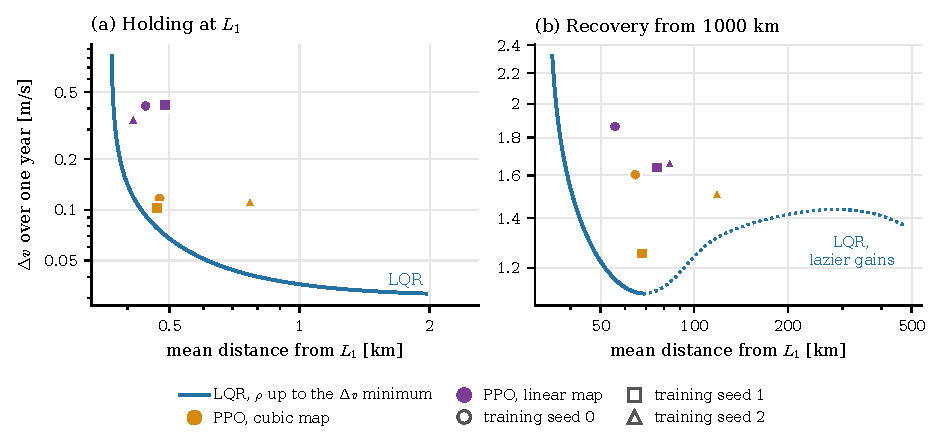
\includegraphics[width=\linewidth]{paper_seed_study}
\caption{PPO models from three training seeds (markers) against the LQR
trade-off on the test seeds (solid: $\rho$ up to the $\dv$ minimum; dotted:
lazier gains, which cost more fuel in recovery). Every model lies above the
LQR curve.}
\label{fig:seeds}
\end{figure}

Table~\ref{tab:ratio} and Fig.~\ref{fig:seeds} show the result. While holding,
the cubic-map agent needs \cubRatioMin--\cubRatioMax$\times$ LQR's fuel at the
same accuracy (mean \cubHoldRatio), the linear map \linHoldRatio. In recovery,
the cubic agent needs \cubAcqRatioMin--\cubAcqRatioMax$\times$ or is dominated.
\textbf{No model, in any training seed or scenario, reaches the LQR curve:
LQR is Pareto-optimal on this problem.}

\subsection{Why the gap shrank: the action representation}

The thrust logs explain the difference between the agents (holding, test
seed 100). LQR's median daily thrust is $\thrLqrMedian$~m/s$^2$, far below
DQN's smallest non-zero action of $10^{-8}$~m/s$^2$. DQN run~1 therefore fires
that smallest level on \dqnOneSmall\ of \thrDays\ days, and run~2 coasts on
\dqnTwoCoast\ days but over-corrects with $10^{-7}$~m/s$^2$ on \dqnTwoMid.
The cubic PPO agent's median thrust is $\thrPpoMedian$~m/s$^2$, almost exactly
LQR's: it has learned the right thrust scale. Its extra fuel comes from the
tail, with \thrPpoBig\ days above $10^{-8}$~m/s$^2$ against \thrLqrBig\ for LQR.
With the linear map the median is $\thrLinMedian$~m/s$^2$ and \thrLinBig\ days
exceed $10^{-8}$~m/s$^2$.

The linear and cubic configurations use the same algorithm, reward and
hyperparameters and differ only in Eq.~\eqref{eq:actionmap}. Across the three
training seeds the linear map needs \linCubHoldMin--\linCubHoldMax$\times$ the
cubic map's holding fuel and \linCubAcqMin--\linCubAcqMax$\times$ its recovery
fuel, with no overlap between the two configurations. Changing only how small
thrusts are represented therefore removes most of the distance between the
learned controllers and LQR, and we conclude that \textbf{most of the DQN--LQR
gap was the action representation, not the learning algorithm}. With the cubic map, the best checkpoint came early in all
three seeds (\cubBestMin--\cubBestMax\ of 3M steps), and longer training never
improved the selection score again; with the linear map the best checkpoints
came late (\linBestMin--\linBestMax\ steps).

\subsection{Robustness outside the training conditions}

All controllers were trained or tuned with the nominal error model and offsets
of at most 1000~km. We pushed them beyond this on the test seeds
(Table~\ref{tab:robust}, Fig.~\ref{fig:robust}): all errors scaled by a factor
$k$, the unmodelled force alone scaled by $k$, and starting offsets of up to
5000~km in four directions. Because the agents can thrust at most
$10^{-6}$~m/s$^2$ and plain LQR has no limit, LQR is also flown saturated at
that limit (``sat.'').

\begin{table}[t]
\centering
\caption{Robustness on the test seeds. Upper part: holding, $\dv$ [m/s] /
RMS distance in the second half of the year [km]; PPO entries are the range
over the three training seeds. Lower part: share of recovery runs kept.
DQN is run~2.}
\label{tab:robust}
\small
\begin{tabular}{lccc}
\toprule
Sweep & LQR & PPO cubic (seeds 0 / 1 / 2) & DQN \\
\midrule
All errors $\times 0$ & 0.00 / 0.0 & 0.00--0.01 / 0.7--1.5 & 0.36 / 2.7 \\
All errors $\times 1$ & 0.06 / 0.6 & 0.10--0.12 / 0.5--0.8 & 0.72 / 1.6 \\
All errors $\times 8$ & 0.50 / 4.9 & 2.02--2.81 / 4.2--4.3 & 5.49 / 9.6 \\
Unmodelled force $\times 100$ & 1.13 / 32.8 & 1.87--2.18 / 6.1--9.6 & 4.10 / 9.6 \\
\midrule
Start 2{,}000 km: kept & 100\,\% (sat.\ 100\,\%) & 100 / 100 / 100\,\% & 65\,\% \\
Start 3{,}000 km: kept & 100\,\% (sat.\ 50\,\%) & 100 / 50 / 50\,\% & 50\,\% \\
Start 5{,}000 km: kept & 100\,\% (sat.\ 50\,\%) & 50 / 50 / 50\,\% & 25\,\% \\
\bottomrule
\end{tabular}

\end{table}

\begin{figure}[t]
\centering
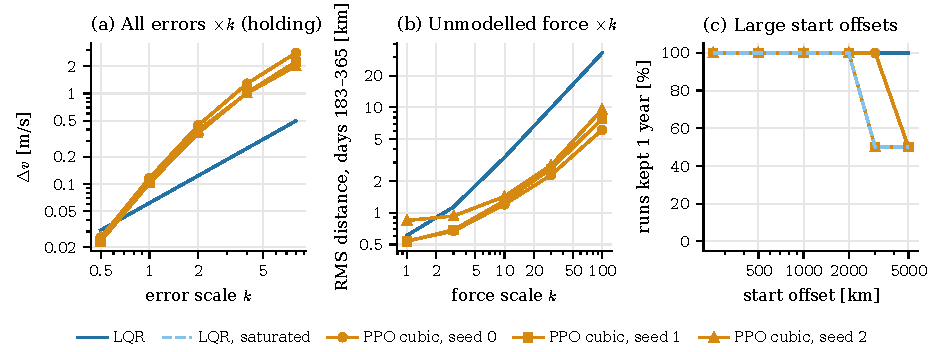
\includegraphics[width=\linewidth]{paper_robustness}
\caption{Robustness on the test seeds for LQR ($\rho = 3$), LQR saturated at
the agents' thrust limit, and the three cubic PPO models. (a) Fuel while
holding as all errors are scaled by $k$. (b) RMS distance in the second half of
the year as only the unmodelled force is scaled. (c) Share of recovery runs
kept from larger starting offsets. Fuel and distance are averaged over the runs
kept.}
\label{fig:robust}
\end{figure}

\paragraph{Noise.} No controller lost a run at up to 8$\times$ the nominal
errors (\noiseLost\ runs lost in the noise and disturbance sweeps). PPO's fuel
overhead grows with the noise, from \noiseOverNomMin--\noiseOverNomMax$\times$
LQR at nominal levels to \noiseOverHiMin--\noiseOverHiMax$\times$ at 8$\times$:
the network reacts to navigation noise, while LQR's response is linear in the
error by construction, so zero-mean noise largely cancels.

\paragraph{Unmodelled forces.} With a 100$\times$ stronger unmodelled force,
LQR with $\rho = 3$ drifts much further out, because its gain was tuned for
nominal conditions, while PPO holds tighter for more fuel. The two now sit at
different points of the trade-off, so neither result is a win.

\paragraph{Large offsets and the thrust limit.} Almost every lost run started
on the Sun--Earth line, the direction of the unstable mode. A rough estimate of
the mode's pull at distance $r$ is $\lambda^2 r$: $\pullThree$~m/s$^2$ at
3000~km and $\pullFive$~m/s$^2$ at 5000~km. At 5000~km it exceeds the thrust
limit, so every bounded controller loses exactly those runs, while unlimited
LQR keeps all of them at a peak thrust of $\lqrPeakFive$~m/s$^2$. At 3000~km
recovery is possible but marginal: saturated LQR, whose gain ignores the limit,
loses \satLostThree\ runs. PPO training seed 0 keeps all of them, at a cost of
about \ppoThreeDv~m/s, and we initially reported this as an advantage of RL.
\textbf{Training seeds 1 and 2 lose exactly the same runs as saturated LQR}, so
this was a property of one training run, not of the method.

% ===========================================================================
\section{Discussion}

\paragraph{Why LQR wins.}
Near $L_1$ the deviations stay below about a thousand kilometres, where the
linearised dynamics are an excellent approximation of the true ones. For
linear dynamics and a quadratic cost, LQR is the optimal state-feedback
controller, and its gain is computed exactly rather than learned from noisy
returns. An RL agent has to rediscover this linear law from samples, through a
reward that only approximates the fuel--accuracy trade-off, and its small
imperfections show up as occasional large thrusts. The setting most
favourable to RL is the strongly nonlinear one, with large offsets near the
thrust limit, but there our only advantage was not reproducible.

\paragraph{The action representation matters more than the algorithm.}
The cubic thrust map is a one-line change in the environment, yet it removed
most of the gap between the learned controller and LQR. We think this is the
most transferable lesson: when the useful actions span several orders of
magnitude, the action parametrisation should make the common, small actions
easy to output.

\paragraph{Single runs can mislead.}
Two of our first-run conclusions did not survive retraining: the fuel ratio
(``1.6$\times$ LQR while holding'' for seed 0 becomes
\cubRatioMin--\cubRatioMax$\times$ across seeds) and the advantage under the
thrust limit, which disappeared entirely. This matches the warnings of
Henderson et~al.\ \cite{henderson2018} and Agarwal et~al.\ \cite{agarwal2021}.
Three seeds are still few; the ranges we report should be read as the minimum
variability, not a confidence interval.

\paragraph{Limitations.}
\label{sec:limits}
The problem is planar and holds the point itself, not a halo or Lissajous
orbit, so the absolute $\dv$ values should not be compared with real missions.
Thrust is a small continuous push updated daily, rather than impulsive
manoeuvres weeks apart. Neither controller uses a state estimator: a Kalman
filter would help both, and would probably help PPO more, since it is the more
sensitive to navigation noise. The RL reward and the LQR cost are different
functions, which is why we compare on the measured fuel--accuracy plane
instead. Finally, we tuned the RL hyperparameters only lightly; better tuning
could narrow the gap, but the agents would still have to beat a controller that
is optimal for the linearised problem.

% ===========================================================================
\section{Conclusion}

On station-keeping at the Sun--Earth $L_1$ point, a classical LQR controller
remains Pareto-optimal on fuel and accuracy against DQN and PPO agents trained
on identical physics and errors. Most of the initial gap between DQN and LQR
came from the coarse discrete action set: with a continuous action and a cubic
thrust map, PPO reaches the right thrust scale and needs
\cubRatioMin--\cubRatioMax$\times$ LQR's fuel at the same accuracy instead of
\dqnRatioMin--\dqnRatioMax$\times$. Natural next steps are halo-orbit
station-keeping in three dimensions, adding a navigation filter to both
controllers, and hybrid designs in which a learned policy corrects a linear
controller only where the linearisation fails.

\section*{Reproducibility}
All code, trained models and raw results are available at
\url{https://github.com/eeymens/l1-station-keeping} under the MIT licence.
\texttt{make reproduce} regenerates every figure and table from the trained
models, and every number in this paper is written into the manuscript by
\texttt{scripts/11\_paper\_assets.py} from the raw CSV files.

\section*{Use of AI tools}
\todo{Describe accurately how AI tools were used (for example, writing parts of
the simulation code and drafting this manuscript) and how you checked the
results. Many venues and competitions require this statement.}

\bibliographystyle{plainnat}
\bibliography{references}

\end{document}
